% --------------------------------------------------------------
% This is all preamble stuff that you don't have to worry about.
% Head down to where it says "Start here"
% --------------------------------------------------------------
 
\documentclass[12pt]{article}
 
\usepackage[margin=1in]{geometry} 
\usepackage{amsmath,amsthm,amssymb}
\usepackage{braket}
\usepackage{graphicx}
\usepackage{calligra}
\usepackage{calrsfs}
\usepackage{subcaption}
\newcommand{\N}{\mathbb{N}}
\newcommand{\Z}{\mathbb{Z}}
 
\newenvironment{theorem}[2][Theorem]{\begin{trivlist}
\item[\hskip \labelsep {\bfseries #1}\hskip \labelsep {\bfseries #2.}]}{\end{trivlist}}
\newenvironment{lemma}[2][Lemma]{\begin{trivlist}
\item[\hskip \labelsep {\bfseries #1}\hskip \labelsep {\bfseries #2.}]}{\end{trivlist}}
\newenvironment{exercise}[2][Exercise]{\begin{trivlist}
\item[\hskip \labelsep {\bfseries #1}\hskip \labelsep {\bfseries #2.}]}{\end{trivlist}}
\newenvironment{reflection}[2][Reflection]{\begin{trivlist}
\item[\hskip \labelsep {\bfseries #1}\hskip \labelsep {\bfseries #2.}]}{\end{trivlist}}
\newenvironment{proposition}[2][Proposition]{\begin{trivlist}
\item[\hskip \labelsep {\bfseries #1}\hskip \labelsep {\bfseries #2.}]}{\end{trivlist}}
\newenvironment{corollary}[2][Corollary]{\begin{trivlist}
\item[\hskip \labelsep {\bfseries #1}\hskip \labelsep {\bfseries #2.}]}{\end{trivlist}}
 
\begin{document}
 
% --------------------------------------------------------------
%                         Start here
% --------------------------------------------------------------
 
%\renewcommand{\qedsymbol}{\filledbox}
 
\title{HW4}
\author{Carl Mueller\\ %replace with your name
CSCI 5254 - Convex Optimization} %if necessary, replace with your course title
\maketitle

\subsection*{5.1)}
\subsubsection*{a}
Feasible set: $\set{x|2 \le x \le 4}$\\
$x^* = 2$\\
$p^* = 5$\\
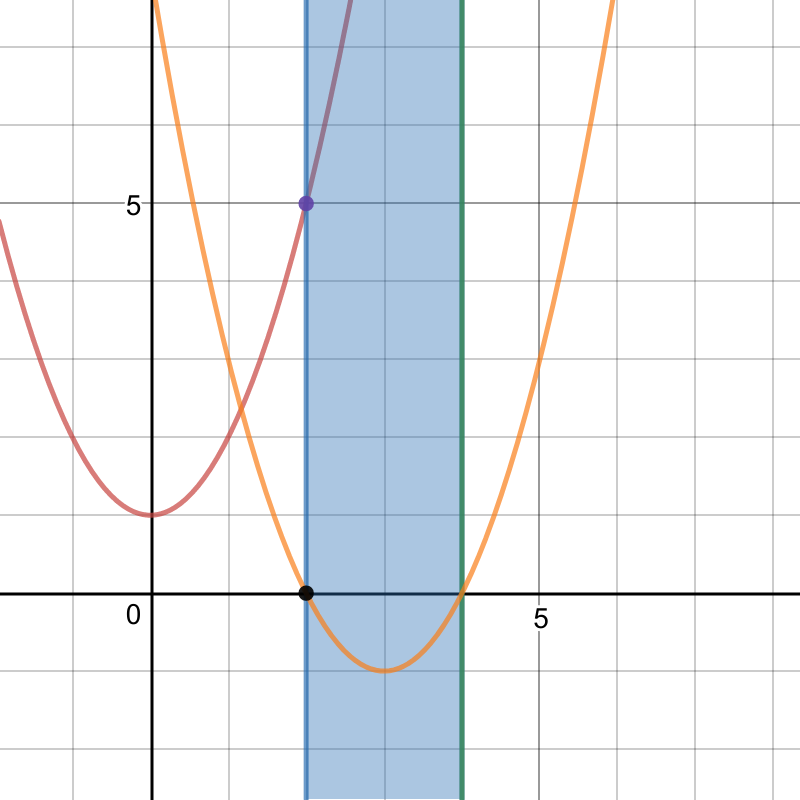
\includegraphics[scale=.25]{1a.png}

\subsubsection*{b}
The Lagrangian:\\
\begin{equation*}
\begin{aligned}
& \mathcal{L}(x,\lambda) = x^2 + 1 + \lambda(x-2)(x-4)\\
& = (1 + \lambda)x^2 - 6\lambda x +  (1 + 8\lambda)
\end{aligned}
\end{equation*}
Gradient w.r.t. x:\\
\begin{equation*}
\begin{aligned}
& \nabla_x \mathcal{L}(x,\lambda)
& = 2x + 2\lambda x - 6\lambda
& = (1 + \lambda)x - 6\lambda  
\end{aligned}
\end{equation*}
Set to zero, solve for x, plug back into lambda to get dual function:\\
\begin{equation*}
\begin{aligned}
& \nabla_x \mathcal{L}(x,\lambda) = (1 + \lambda)x - 6\lambda  = 0\\
& x = \frac{3\lambda}{1+\lambda}\\
& g(\lambda) = inf(\frac{-9\lambda^2}{1-\lambda} + 8\lambda + 1)
\end{aligned}
\end{equation*}

\begin{figure}[h]
    \begin{subfigure}[h]{0.5\textwidth}
        \centering
        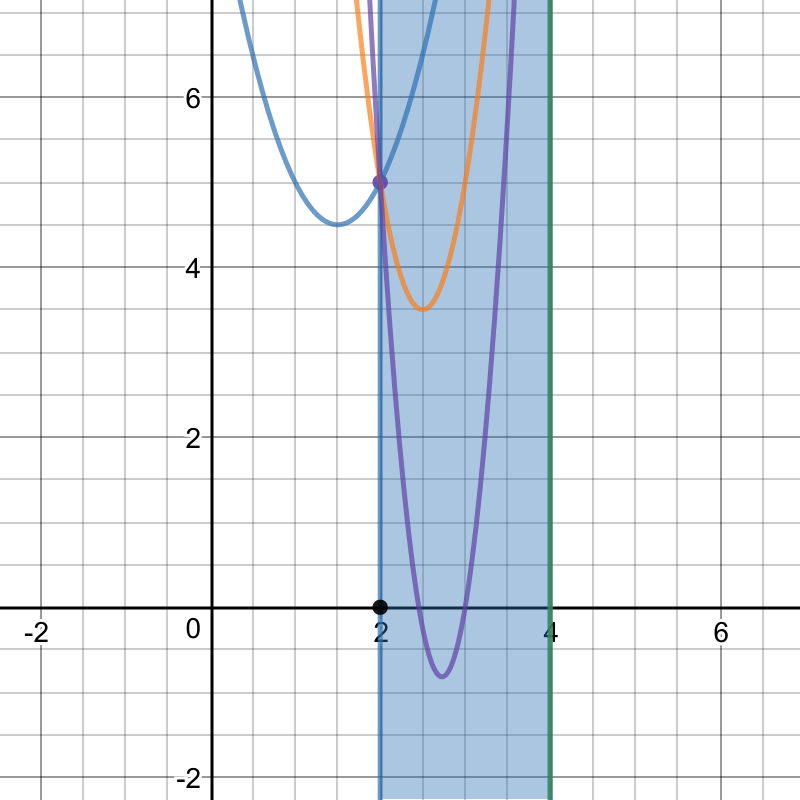
\includegraphics[scale=.25]{1b.png}
    \end{subfigure}
    \begin{subfigure}[h]{0.5\textwidth}
        \centering
        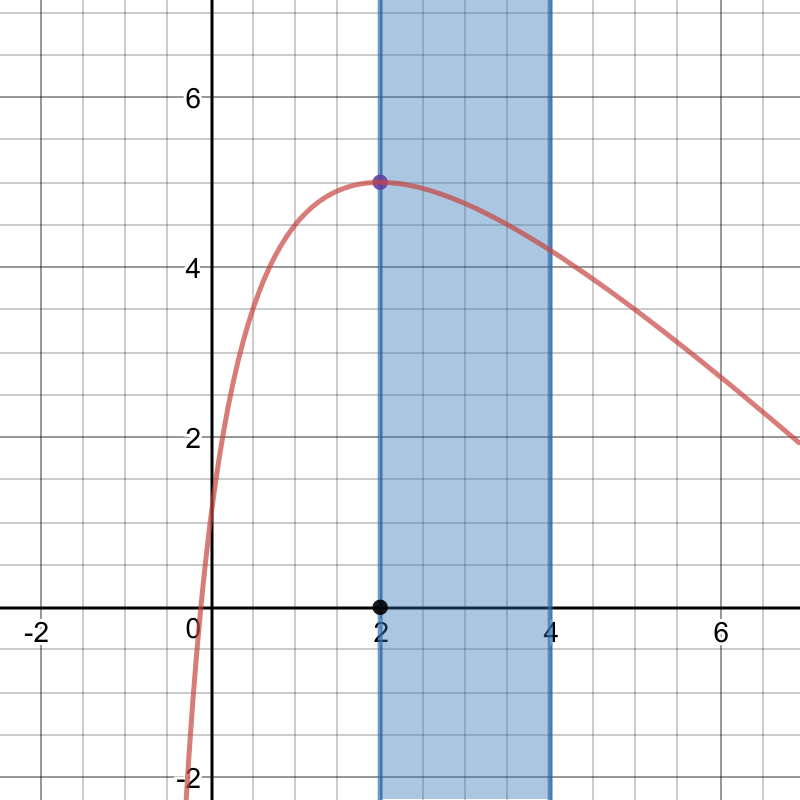
\includegraphics[scale=.25]{1b_2.png}
    \end{subfigure}
\end{figure}

\subsubsection*{c}
The dual problem:
\begin{equation*}
\begin{aligned}
& \underset{\lambda}{\text{maximize}}
& & \frac{-9\lambda^2}{1-\lambda} + 8\lambda + 1\\
& \text{subject to}
& & \lambda \ge 0\\
\end{aligned}
\end{equation*}
Take the gradient of the dual w.r.t. $\lambda$, set to zero, to show strong duality:\\
\begin{equation*}
\begin{aligned}
& \nabla_x g(\lambda) = 0\\
& \frac{-9\lambda (1-\lambda)+9\lambda^2}{(1+\lambda)^2} + 8 = 0\\
& -9\lambda (1-\lambda)+9\lambda^2 + 8(1+\lambda)^2 = 0\\
& \lambda^2 + 2\lambda - 8 = 0\\
& (\lambda + 4)(\lambda - 2) = 0\\
& \text{$\lambda$ must be greater than 2:}\\
& \lambda \not= -4, \lambda = 2\\
& 5 = p^* = g^* = g(2) = 5 
\end{aligned}
\end{equation*}

\subsection*{5.11)}
\begin{equation*}
\begin{aligned}
& \underset{\lambda}{\text{minimize}}
& & \sum_{i=1}^{N}||A_ix+b_i||_2 + \frac{1}{2}||x-x_o||_2^2\\
& \text{subject to}\
& & y_i = A_ix+b_i\\
\end{aligned}
\end{equation*}
The Lagrangian:
\begin{equation*}
\begin{aligned}
& \mathcal{L}(x,y, \lambda_1 \dots \lambda_N) = \sum_{i=1}^{N}||y_i||_2 + \frac{1}{2}||x-x_o||_2^2 + \sum_{i=1}^{N}\lambda_i^T(y_i-A_ix+b_i)\\
& = \sum_{i=1}^{N}||y_i||_2 -\lambda_i^Ty_i + \frac{1}{2}||x-x_o||_2^2 - \sum_{i=1}^{N}\lambda_i^T(A_ix+b_i)\\
\end{aligned}
\end{equation*}
Minimize w.r.t. y:
\begin{equation*}
\begin{aligned}
& inf(\sum_{i=1}^{N}||y_i||_2 -\lambda_i^Ty_i + \frac{1}{2}||x-x_o||_2^2 - \sum_{i=1}^{N}\lambda_i^T(A_ix+b_i))\\
& = \sum_{i=1}^{N}inf(||y_i||_2 -\lambda_i^Ty_i + \frac{1}{2}||x-x_o||_2^2 - \lambda_i^T(A_ix+b_i))\\
& \text{Based on Cauchy-Schwarz Inequality: }\\
& = \begin{cases}
    \frac{1}{2}||x-x_o||_2^2 - \lambda_i^T(A_ix+b_i) & \text{if } ||\lambda||_* \le 1\\
    -\infty & \text{otherwise}
    \end{cases}\\
\end{aligned}
\end{equation*}
Constraint on dual is $$||\lambda||_* \le 1$$
Minimize w.r.t. x via gradient and then set to zero:
\begin{equation*}
\begin{aligned}
& \nabla_x(|\frac{1}{2}||x-x_o||_2^2 - \sum_{i=1}^{N}\lambda_i^T(A_ix+b_i)) = 0\\
& x-x_o - \sum_{i=1}^{N}\lambda_i^TA_i = 0\\
& x = x_o - \sum_{i=1}^{N}\lambda_i^TA_i
\end{aligned}
\end{equation*}
Plug into Lagrangian to get dual function:
\begin{equation*}
\begin{aligned}
& g(\lambda_1, \dots, \lambda_N) = \sum_{i=1}^{N}(A_ix_o + b_1)- \frac{1}{2}||\sum_{i=1}^{N}A_i^T\lambda_i||^2
\end{aligned}
\end{equation*}
The Dual Problem:
\begin{equation*}
\begin{aligned}
& \underset{\lambda}{\text{Maximize}}
& & \sum_{i=1}^{N}||A_ix+b_i||_2 + \frac{1}{2}||x-x_o||_2^2\\
& \text{subject to}\
& & y_i = A_ix+b_i\\
\end{aligned}
\end{equation*}
% --------------------------------------------------------------
%     You don't have to mess with anything below this line.
% --------------------------------------------------------------
 
\end{document}